% This is a sample document using the University of Minnesota, Morris, Computer Science
% Senior Seminar modification of the ACM sig-alternate style. Much of this content is taken
% directly from the ACM sample document illustrating the use of the sig-alternate class. Certain
% parts that we never use have been removed to simplify the example, and a few additional
% components have been added.

% See https://github.com/UMM-CSci/Senior_seminar_templates for more info and to make
% suggestions and corrections.

\documentclass{sig-alternate}
\usepackage{color}
\usepackage[colorinlistoftodos]{todonotes}

%%%%% Uncomment the following line and comment out the previous one
%%%%% to remove all comments
%%%%% NOTE: comments still occupy a line even if invisible;
%%%%% Don't write them as a separate paragraph
%\newcommand{\mycomment}[1]{}

\begin{document}

% --- Author Metadata here ---
%%% REMEMBER TO CHANGE THE SEMESTER AND YEAR AS NEEDED
\conferenceinfo{UMM CSci Senior Seminar Conference, December 2015}{Morris, MN}

\title{Concurrent Compaction in JVM Garbage Collection}

\numberofauthors{1}

\author{
% The command \alignauthor (no curly braces needed) should
% precede each author name, affiliation/snail-mail address and
% e-mail address. Additionally, tag each line of
% affiliation/address with \affaddr, and tag the
% e-mail address with \email.
\alignauthor
Jacob P. Opdahl\\
	\affaddr{Division of Science and Mathematics}\\
	\affaddr{University of Minnesota, Morris}\\
	\affaddr{Morris, Minnesota, USA 56267}\\
	\email{opdah023@morris.umn.edu}
}

\maketitle
\begin{abstract}
This paper provides a basic overview of both garbage collection (GC) 
of memory and parallel processing. We then cover how 
parallel processing applies to GC. Particularly, these
concepts are focused within the context of the Java Virtual Machine (JVM).
With that foundation, we look at various algorithms that perform compaction of fragmented 
memory during the GC process. These algorithms are designed 
to run concurrently to the application running.
Such concurrently compacting GC behavior stems from a desire to reduce stop-the-world
pauses of an application.
% The current paper format *only* allows inline comments using the todo
% macro. That's kind of a bummer, and it would be neat if someone figured
% out how to change the acmconf style to allow this. I suspect it isn't *hard*
% but there are quite a few details that have to be sorted out in synchrony.
\end{abstract}

\keywords{garbage collection (GC), concurrency, compaction, Continuously Concurrent Compacting Collector (C4), Collie, Field Pinning Protocol (FPP)}


\section{Introduction}
\label{sec:introduction}

In programming languages, the allocation and deallocation
of memory for objects can be explicit or implicit. If done implicitly,
a language is said to have \emph{automatic memory management}. Some languages 
with automatic memory management are C\#, Java, and Python.
Use of automatic memory management is beneficial to programmers as it 
prevents them from worrying about the details of memory allocation and deallocation. 
However, programmers also do not have control over how memory management occurs,
which can have negative impacts on application performance.

Since memory for a program is not an unlimited resource, automatic memory management
must remove unused objects from memory when appropriate.
Dead objects, or \emph{garbage}, are objects that can be shown
to be unreachable by the program~\cite{glossary:g}. Garbage should be deallocated to 
save space for new objects that will be created. The algorithm used to perform implicit
deallocation of garbage is referred to as a \emph{garbage collector}.
A garbage collector is an algorithm designed to detect
and remove dead objects. We will focus on
garbage collection (GC) performed on Java Virtual Machines 
(JVMs), software processes that run programs written in Java and other languages 
on computing systems~\cite{Lindblom:2011}.

GC is not without cost.
Just like the application, GC requires processing resources to run. When using a single processor, 
we get a \emph{serial} garbage collector operating in a 
\emph{stop-the-world} fashion~\cite{Lindblom:2011}; GC requires
pausing the application in order to clean. 
Growing storage media is leading to more memory
availability for programs, which means garbage collectors
have more garbage to remove. Thus, stop-the-world pauses
experienced by applications are increasing.

In some environments,
application pauses are unacceptable; for example, see the section on 
real-time GC in~\cite{Lindblom:2011}. In order to decrease or remove 
pauses, we want to use multiple
processors to share the workload of both running an application and its GC.
This is known as \emph{parallel processing}, and it can be used
to enhance performance of both. With
demand for faster responding applications coupled with more memory needing managing,
it is paramount that GC be optimized using parallel processing. 

In Section 2, we go over background information for GC, parallel processing,
and a combination of the two.
From there, we focus our examination of parallel processing in GC.
Section 3 covers the Continuously Concurrent Compacting Collector (C4), Section
4 considers the Collie collector, and Section 5 looks at the Field Pinning Protocol (FPP).
Discussion of each is focused on how one component of GC can run parallel to
and independent of the application running. 


\section{Background}
\label{sec:background}


\subsection{Garbage Collection (GC)}
\label{sec:garbageCollection}

Newly allocated objects in JVM languages are stored in a contiguous memory location referred
to as the \emph{heap}~\cite{oracle:heap}. The heap represents the memory available to a program.
Thus, when GC removes garbage, it cleans the heap.
An application accesses objects stored on the heap through \emph{references},
fixed-size values that refer to object locations in the heap~\cite{reilly:reference}. 
As such, an application process never stores
an actual object. It stores references to objects in a memory structure known
as the \emph{stack}, which is separate from the heap.
The heap is a virtual layer of memory that corresponds to physical memory.
References pointing to object locations actually point to their
virtual locations rather than their physical locations. Objects may also 
contain references to other objects, so references may appear on the heap.

In GC, the overarching pattern common to all algorithms is determining garbage
and reclaiming memory from dead objects. This can be broken down into two major steps.
First, a GC algorithm performs \emph{set condemnation} when deciding which objects are 
garbage. The garbage collectors we examine perform set condemnation using a method 
known as \emph{tracing}. During this, objects are determined to be reachable by 
traversing references from global, root objects. Any objects reachable by chaining references
from these global, root objects could still be used by the application. 
Any objects not reachable are garbage. Then, the algorithm performs 
\emph{reclamation} by recovering the memory held by garbage objects. A full
performance of the overall GC pattern is known as a \emph{cycle}, and it
is usually started when the heap is full.

To optimize GC, a variant can be performed known as \emph{generational} GC.
Generational collectors are based on the \emph{weak generational hypothesis}~\cite{Tene:C4}.
This says most objects do not live on the 
heap long. Thus, GC efforts are focused on these objects. Typically, this is achieved
by dividing the heap into two generations. One generation focuses on the younger objects and
is collected more frequently. If objects in the young generation of the heap survive
enough GC cycles, it will move into the old generation. By not considering the entire
heap with each GC cycle, an application experiences less disruptions.

As memory is reclaimed by a garbage collector, the heap is subject to 
\emph{fragmentation}~\cite{Tene:C4}~\cite{Iyengar:Collie}~\cite{Osterlund:FPP}. Fragmentation is the forming
of interspersed locations of used space in contiguous memory. This
is an issue as space for new objects being allocated
on the heap becomes difficult to find and manage. 

For example. Assume
we have an object that takes 4MB of memory. After several cycles of GC,
we have gaps of open memory with a size of at most 2MB contiguously. Thus, 
the JVM experiences additional overhead in allocating space for this object
as it has to store parts of it across non-contiguous locations. Additionally,
more overhead will be experienced as accessing the object will require locating
all of its parts.

This is where \emph{compaction} becomes relevant. Compaction fights
fragmentation of the heap by moving lives objects into contiguous memory locations.
Compaction is performed by a garbage collector and is part of GC. Two steps
are typically involved in compaction. \emph{Relocation} occurs by moving live objects
to a contiguous memory location after set condemnation.
The contiguous memory location being moved to is often referred to as \emph{to-space}.
The location an object is moved from is referred to as \emph{from-space}. While it is called 
relocation, objects are typically copied rather than moved. \emph{Remapping}
occurs after objects have been relocated; the remapping phase 
updates all references to moved objects to refer to their new locations. Often, reclamation
in compacting collectors is performed by marking from-spaces as freed.


\subsection{Parallel Processing Basics}
\label{sec:parallelProcessing}

To develop an understanding of parallel processing, we need to know 
what \emph{processes} and \emph{threads} are~\cite{oracle:threads}.
A process is an instance of a computer program being run. What we
see as an application being run can actually incorporate multiple processes.
For example, a Java application being run and GC being performed on the application are two processes.
A thread, at a basic level, is a component of a process. A thread performs a sequence
of instructions that are part of a process the thread belongs to. In JVM languages,
each thread has a personal stack to keep track of variables
and references used within its specific set of tasks. A process
can involve a single thread or multiple threads.
Parallel processing is the utilization of multiple
cores of a CPU to run threads concurrently. If processes are set up
to run with multiple threads, the extra processing power can be used to make 
the process more efficient.

% Could make an image for this example if needed and space allows.
% HOnestly, this whole paragraph could possibly be removed too...
%If I do, remove the last sentence of the preceding paragraph too.
If parallel processing makes running processes more efficient, why is it not
always used? The reason is creating parallel processes subjects
developers to new challenges. Many new issues can result from use of
multi-threading. One example, relevant to GC, is modifications to an 
object can be lost. For example, say there is an application keeping 
track of people's moods and locations. People are stored as objects. 
Thread 'a' moves people, and it does so by relocating them in data structures (DSs) 
with a deep copy and delete operation. Thread 'b' updates people's moods. Suppose a person
is about to go home from work, so their mood changes to happy.
The person's change in mood could be lost if thread 'a' copies the person
to the home DS, thread 'b' updates the person's mood while still expecting
them to be in the work DS, and thread 'a' deletes the person from the work DS. 
While the example is fairly simple, it can be seen how this type of problem
applies to GC.

To deal with multiple threads relying on use of the same data, \emph{synchronization}
techniques are used. These ensure threads do not interfere
with one another in a process-breaking manner. A \emph{memory barrier} (referred to 
as a read barrier or simply barrier) is an instruction set enforced upon the 
CPU to be performed before accessing memory~\cite{wiki:barrier}. Uses of this include ensuring threads
meet certain requirements before accessing memory or disallowing a thread to
access memory while another thread is using the memory.
 
A \emph{checkpoint} is a technique
where all threads are required to pass through a barrier-like function at some point
during an overall process~\cite{Tene:C4}. Going back to our moods and locations example, say we
now have multiple threads in charge of relocating people. These threads
could be required to store a flag on their stacks when relocating a person.
When thread 'b' tries updating someone's mood, all threads go through
a barrier function checking if there is a flag for relocating that person. This
could prevent thread 'b' from updating a person's mood while they are being relocated.


\subsection{GC with Parallel Processing}
\label{sec:parallelProcessingGarbageCollection}

We can now return to our original goal of applying parallel processing to GC.
Threads that are part of the application process are referred to as \emph{mutator}
threads (or mutators) because they mutate the data~\cite{Tene:C4}~\cite{Iyengar:Collie}
\cite{Osterlund:FPP}. Threads used by the garbage collector are simply GC threads.

A \emph{parallel} garbage collector is one using
multiple threads simultaneously to complete its GC process.~\cite{Puffitsch:background}
All but one of the garbage collectors we examine are parallel. A \emph{concurrent} garbage
collector is one executing in parallel to the application running. In other 
words, the garbage collector does not entirely stop-the-world. A GC algorithm
could be only partially concurrent or parallel. For example, one collector may
only have the tracing phase be parallel while reclamation is concurrent.

We focus on three techniques for performing
concurrent compaction within GC. We do so due to the importance 
of having non-stop-the-world garbage collectors. Additionally, compacting
collectors are vital when trying to optimize application performance. Thus,
the intersection of these two optimizations to languages with automatic memory management leads
to researching ways to perform concurrent compaction within GC.

All compaction techniques we examine are used in garbage
collectors for testing purposes. One important metric used to consider
how a collector is affecting an application is \emph{latency}~\cite{Lindblom:2011}.
Within GC, latency is a measure how much a collector negatively impacts
application processing performance. A higher latency implies the collector
is taking up more processing resources that the application could be using. It 
can be measured in various ways and is usually collected in the same manner
among multiple collectors for comparative purposes.


\section{The C4 Collector}
\label{sec:c4}

The first concurrent compaction algorithm we examine is implemented in the 
Continuously Concurrent Compacting Collector (C4), which is a garbage collector 
included in JVMs commercially shipped by Azul Systems~\cite{Tene:C4}. The 
researchers, Iyengar et al., describe how C4 is an enhanced, generational variant
of the Pauseless Garbage Collector~\cite{Click:Pauseless}. C4 is generational in 
that the entire GC algorithm is independently utilized in both the young and old generations;
in addition, both generations are concurrent with the application. 
For set condemnation, C4 uses a tracing-style algorithm.
C4's intended environment is large servers with multiple gigabyte heaps.


\subsection{Loaded Value Barrier}
\label{sec:c4LVB}

\begin{figure}
\centering
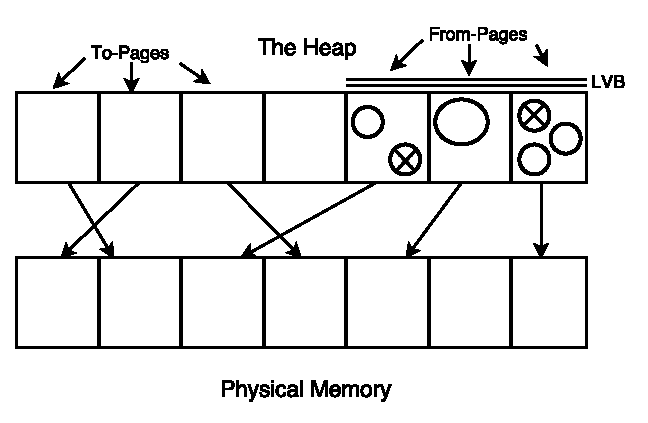
\psfig{file=c4_page_rough_2.pdf,width =3in}
\caption{Simplified representation of memory management with C4. Memory is relocated
page-by-page. Dead objects are represented with $X$ and will not be relocated.
From-pages are protected from mutators by the LVB. Contiguous virtual memory
may not correspond to contiguous physical memory, which is out of our scope of discussion.}
\label{fig:c4Memory}
\end{figure}

C4 uses a read barrier referred to as the \emph{Loaded Value Barrier} (LVB) to 
maintain synchronization of concurrent threads throughout the GC process~\cite{Tene:C4}. The LVB 
places invariants on each reference as it is loaded from memory.
One of the invariants relates to the tracing portion of the GC algorithm, so
it is not discussed here. The other invariant ensures
references loaded by a mutator during relocation must point to safely
accessible objects, objects that have already been moved.
If the invariant does not hold
when a reference is loaded, the barrier will trigger and execute code to correct
the situation.


\subsection{Concurrent Relocation}
\label{sec:c4Relocation}

The relocation phase of compaction in C4 occurs on a per-\emph{page}
basis, where a page is a fixed-length, contiguous block of virtual memory in the heap
backed by a contiguous block of physical storage~\cite{Tene:C4}.
To quickly empty pages, the most sparsely populated ones are relocated
first. In the case of Figure~\ref{fig:c4Memory}, the left-most 
\emph{from-page}, analogous to from-space, is relocated first as it has only one small object alive.
The object is copied to a \emph{to-page}, which is analogous to to-space.

From-pages are protected by the LVB as can be seen in Figure~\ref{fig:c4Memory}. 
LVB will trigger for mutator threads encountering a reference to an object
on a protected page. The mutator's subsequent behavior is:
\begin{itemize}
\item If the object is relocated already, find its new location
\item If the object is being relocated currently, wait until the GC thread is finished
\item If the object has not been relocated, move the object 
\end{itemize}
In all cases, the mutator cannot use the object until it is on a to-page.
Additionally, LVB has mutators correct the
references to avoid further barrier triggers on the same
reference.
Without mutator interference, GC threads will simply relocate the objects but
not remap references at this time. 

When all live objects are relocated from a from-page,
the C4 compactor will perform \emph{quick release}. 
The physical memory backing the page will be freed
once the last live object has been moved to a to-page. The objects have already 
been transferred to new pages, so the contents of the from-pages are no longer needed. The from-page 
will be in use as it still has references to it, but the physical memory can be recycled efficiently. 
In terms of Figure~\ref{fig:c4Memory}, the heap
memory seen on top is in use until after the remapping phase, but the physical memory below 
can be paired with a different virtual page and used immediately.


\subsection{Concurrent Remapping}
\label{sec:c4Remapping}

To maintain concurrency while updating all references to the now relocated
objects, the C4 compaction algorithm uses two techniques~\cite{Tene:C4}. The first is
\emph{lazy remapping}. With this, mutator
threads continue updating references as they trigger the LVB. In order for
the remapping phase to end, all live references must be updated.
This could go on indefinitely if lazy remapping alone is performed.

To finish remapping, a traversal of live references must be performed to
ensure all are updated; this is like the traversal performed to trace which
objects are garbage. Since no physical resources are being held due
to quick release and lazy remapping does not severely impact mutator operations,
the remapping traversal is delayed until another GC cycle starts.
C4 will perform the remapping of one GC cycle while the tracing
of another cycle is beginning. This works as both processes need to traverse
the same references in memory. To
visualize how this works, examine Figure~\ref{fig:c4Cycle}. Upon remapping completion, 
all references to from-pages are now gone. Thus, the virtual addresses
are freed and reclamation of memory is now complete. 

\begin{figure}
\centering
\psfig{file=c4Mapping_rough_figure_3.pdf,width =3in}
\caption{C4 GC cycle. Remapping and Tracing are rolled into one traversal.
(taken from \cite{Tene:C4})}
\label{fig:c4Cycle}
\end{figure}


\subsection{C4 Results Summary}
\label{sec:c4Results}

% Tested primarily against also concurrent, but non-generational.

Experiments done with the C4 collector were meant to show improvements
of using an algorithm that is simultaneously generational and concurrent~\cite{Tene:C4}.
C4 is tested against a modified, non-generational C4 algorithm as well as
two algorithms that do not perform concurrent compaction. 
All GC algorithms were tested on the same hardware; for specifications, see~\cite{Tene:C4}. 
The test exhibited live sets of objects on 
the heap consistently at a size of around 2.5 gigabytes (Gbs); the actual heap size was allowed 
to grow, indicating greater amounts of garbage on the heap. The applications were run long
enough to ensure multiple full-heap GC cycles ran and at least one
significant compaction event occurred.

The primary performance metric monitored was worst-case response times
of servers while experiencing the heap sizes
described. While not directly measuring latency, this gives a sense of how 
much latency a garbage collector causes. 
C4 maintained the smallest 
worst-case response times across the largest range of heap sizes.
The worst-case response times were usually in the range of 0.01-0.1 secs. 
The non-generational version of C4 could also reach low worst-case response times,
but for a more limited range of heaps sizes. Standard
C4 sustained the times for heap sizes of 5-35 Gb; the modified C4 could
only do so for heaps sizes of 15-35 Gb. The non-concurrently compacting
collectors had multi-second worst-case response times for all heap sizes.


\section{The Collie Collector}
\label{sec:collie}

We now look at the concurrent compaction technique used by the single-threaded
Collie garbage collector described by Iynegar et al.~\cite{Iyengar:Collie};
with the exception of Gehringer, they were the researchers who worked on C4.
As such, Collie utilizes modified versions of several techniques from C4, such as:
the tracing algorithm, the LVB, page-granularity compaction, and quick-release behavior.
Only the LVB is modified in significant ways as discussed below.
Like C4, the Collie
collector is also designed with server environments in mind. 
Collie is implemented and tested in 
the same production-quality Azul JVM the Pauseless garbage collector is implemented in
~\cite{Click:Pauseless}. However, it is not commercially available.


\subsection{Transactional Memory}
\label{sec:collieTM}

The Collie's compaction algorithm sets itself apart due to use 
of a \emph{transactional memory} (TM) system as a concurrency control 
alternative to barriers~\cite{Iyengar:Collie}. TM systems allow
sections of code to function 
analogously to \emph{transactions} from database systems, 
which are a series of operations performed as one unit where 
they occur in an all-or-none manner.

For example, consider updating sale prices of items in a store; this requires
ensuring the store price matches the sale price advertised. 
If a person updates the prices for an item, they want both the
advertised price and the store price to be updated. Only updating the
advertised price could lead to irate customers, and only updating the
store price could lead to customers not knowing about the sale. A transaction
ensures an item's prices are unchanged if the update process 
is started and then aborted before completion.

% Might be too much detail. Consider cutting later.
TM systems allow a series
of operations modifying memory to be placed in
a \emph{transactional procedure}, much like a database transaction.
The TM system then monitors the access of concurrent threads to \emph{transactional variables},
memory modified by a transactional procedure.
Concurrent threads will operate in parallel until they try to modify
the same transactional variable. At this time, how 
the conflict should resolve can be specified, but the general behavior would be for one transaction
to be aborted and the other allowed to continue.
When a transaction is completed, its changes are \emph{committed}; any changes 
made to memory by the transaction are finalized~\cite{wiki:transactional-memory}.


\subsection{Referrer Sets}
\label{sec:collieReferrerSets}

Each object on the heap has a \emph{referrer set}. This is the precise set 
of all references pointing to the object. Collie stores object's referrer sets
so that it can perform a single object's relocation and remapping as a transaction.
To ensure an object's referrer set is not modified during the transaction,
we define a \emph{stable} referrer set. An object has a stable referrer 
set if the object's referrer set meets the following criteria:
\begin{enumerate}
\item Once the overall GC process begins, no references to the object may be written to the heap
\item At the start of the object's transplantation, no threads contain references to the object in their stacks
\item Once transplantation is underway, no new references may be added to the object's \emph{transplantation state} until it is complete
\end{enumerate}
This ensures the compactor is aware of all references to the object
and references to the object go unchanged.


\subsection{Aborting Compactor}
\label{sec:collieAbortion}

Mutator threads interrupting the transaction for relocating and remapping
an object or triggering the modified LVB will cause the object to go unmoved.~\cite{Iyengar:Collie}.
However, unmoved objects due to these abortions would then be stuck
in from-space. This is why
the additions of a \emph{mirrored-to-space} and \emph{zero-copy transplantation} are necessary.

% THere's definitely some repition here. Worry about later.
Mirrored-to-space is a virtual address space that corresponds to and is the same
size as from-space. Mirrored-to-space memory pages are mapped to the same physical
memory as their corresponding from-space pages. For barrier test and compaction 
termination purposes, mirrored-to-space is logically considered part of to-space.

Mirrored-to-space is necessary to facilitate non-compacting, zero-copy transplantation 
between from-space and to-space. An object's contents are 
consistent between from-space and mirrored-to-space and mirrored-to-space
is logically considered to be to-space. Thus, transplantation to "to-space"
can be done without copying the object's contents. That is, zero-copy transplantation
allows transplantation of an object from from-space to mirrored-to-space, which only
requires correcting references. The purpose of this is to ensure
an object makes it to "to-space" should its transplantation need 
to be aborted because mutators need to access it.

\todo[inline]{Add figure to clarify here!!}


\subsection{The Collie Protocol}
\label{sec:collieProtocol}

After a tracing phase at the start of the overall GC algorithm for set condemnation, heap compaction
happens during a \emph{transplantation phase}~\cite{Iyengar:Collie}.
Live, relocatable objects and their referrer sets are known at this time. The compaction 
algorithm uses TM semantics to complete an object's
transplantation. The operations for transplantation are stored as a
transactional procedure. Individual object transplantations will be done on relocatable objects 
maintaining stable referrer sets throughout the process.

An object is deemed \emph{non-individually transplantable} (NIT) if its transplantation
has to be aborted or if it fails to maintain a stable referrer set. 
Any object deemed as such will be moved to mirrored-to-space by zero-copy 
transplantation. An object may be declared NIT during the tracing phase before transplantation
if it violates requirement 1 for having a stable referrer set; discussion
of how this occurs is beyond the scope of this paper, see~\cite{Iyengar:Collie}.

% Talk about this barrier because it is during GC - betweentracing and transplantation.
% If others experience something similar, they should be talked about too.
At the start of the transplantation phase, a pre-compaction checkpoint occurs.
For all relocatable objects, referrer sets have been established during the tracing phase.
These referrer sets need to be stable referrer sets. As such, threads' stacks are checked 
for references to the objects. Any objects with these will be 
marked NIT as their referrer sets fail to meet requirement 2 for being stable referrer sets.
After the checkpoint, the compactor has a set of relocatable objects with currently stable referrer sets.

The pre-compaction checkpoint also kicks off the LVB-style read barrier's first purpose. 
The barrier will trigger on the load of a reference to an object that was 
relocatable. Upon being triggered, the object will be marked NIT. This is done because
the load operation adds another reference to the object's referrer set, which violates
requirement 3 of having a stable referrer set.

With the set of objects to be transplanted, the compactor uses transactional
procedures to complete the individual object transplantations to to-space.
The copying of an object occurs outside the transaction since any
mutator access of the object will trigger the LVB-style read barrier,
rendering the object NIT. Thus, only the referrer set updating
is done in the transactional procedure. The transaction looks like:
\begin{enumerate}
\item Transaction is started
\item References are checked to make sure none point to the mirrored-to-space location as this means the object had been changed to NIT by some previous, interrupting operation
\item All references are changed to point from an object's from-space location to its new to-space location
\item Memory transaction is committed
\end{enumerate}
If a transaction fails or is interrupted, as detected by the TM system, then the object is rendered NIT.

After the transactional procedure either succeeds or fails for the 
relocatable objects with stable referrer sets, all that remains is to perform zero-copy transplantation
on all NIT objects. Just like the C4 compactor, Collie will do this lazily. This is the second purpose
of the LVB-like barrier; as mutators try to access NIT objects before their references are updated to
point to mirrored-to-space, the barrier will force them to correct the references. Also like C4, Collie
rolls the full traversal of memory to finish zero-copy transplantation of all NIT objects into the next
tracing phase.


\subsection{Collie Results Summary}
\label{sec:collieResults}

% Tested primarily against Another concurrent that is also modified to run on a single thread.

The main goal of the Collie collector is to decrease latency
during compaction~\cite{Iyengar:Collie}. The Collie was tested 
against a modified variant of the Pauseless collector~\cite{Click:Pauseless}.
Accordingly, both collectors were implemented on the same JVM. For hardware
specifications used for testing, refer to~\cite{Iyengar:Collie}. The Collie
utilizes several aspects of the C4 collector, which in turn builds upon the Pauseless
collector. This provides an effective comparison to see how the main differences, 
use of transactional memory and an aborting compactor, affect application performance. 

To examine latency, \emph{minimum mutator utilization} (MMU) is measured.
MMU is the minimum percentage of mutators being utilized over a period of time~\cite{Bacon:MMU}. Ideally,
MMU would always be at 100\% so all mutators are being used. 
MMUs were taken from various time periods during which
compaction was running and was compared between the two algorithms. Comparisons were done
with a 128MB heap and a 512MB heap. For all time windows, the Collie compactor
had higher MMUs than Pauseless. Collie did not go below a 70\% mutator utilization 
level whereas Pauseless ranged over the whole spectrum of values. 
This shows the aborting nature of Collie
lends itself to ensuring mutator response time, and thus decreasing latency, 
despite potentially limiting the amount of memory compacted.


\section{Field Pinning Protocol}
\label{sec:fpp}

Last, we examine concurrent compaction in GC through the Field Pinning
Protocol, (FPP) designed by \"{O}sterlund and L\"{o}we~\cite{Osterlund:FPP}.
FPP describes a lock-free process for performing the relocation aspect
of concurrent compaction. The remapping phase as well as other portions
of GC are left up to the host garbage collector this
protocol is implemented within. FPP is compliant with the Java Native Interface
to allow for integration into a JVM. For purposes of testing, FPP 
is implemented within the Garbage-First GC algorithm in the HotSpot JVM 
of OpenJDK 9~\cite{Detlefs:G1}.


\subsection{Hazard Pointers}
\label{sec:fppHazard}

The key component driving FPP is the \emph{hazard pointer} (HP)~\cite{Osterlund:FPP}. 
In FPP, all mutator threads contain a list of HPs.
The HPs point to objects in memory a thread is accessing, or \emph{pin} them.
When a thread finishes using an object, it drops the HP.
So long as an object
is pinned by a mutator, it cannot be relocated as it is still in use. Once all threads have
unpinned the object, it can safely be relocated.
When discussing the theoretical construction of the algorithm, a granularity of pinning 
individual fields is used, thus the name \emph{Field} Pinning Protocol. 

% Changed from original example using cake. May want to change back depending
% on reader feedback. Cake at a party.
While it is explained in more detail below, an example of how HPs 
work on a high-level is useful. Imagine a pot of coffee at work. Anyone 
wanting coffee must make it known to others by having a cup, otherwise the 
coffee is liable to be moved to another break room. The people are effectively pinning the coffee.
Once everyone has had their share of caffeine, it should be moved. This can
be done safely when no one has cups any longer, so the coffee is not pinned.

% Took out from this example that last person to discard the cup will be responsible.
% Did so to be able to build on the example.


\subsection{Collaborative Copying and Blame}
\label{sec:fppCopy}

HPs prevent premature relocation of objects by serving as a distributed
counter. Threads cannot relocate objects if the number of
HPs pinning the objects is greater than zero.
A mutator thread \emph{impedes} a copying thread if
its HP prevents the copying.
The impeding thread is \emph{blamed} for the 
interruption~\cite{Osterlund:FPP}; it becomes responsible for ensuring 
the object is relocated. GC threads cannot receive blame as they will not impede
copy attempts.

The process followed by mutator threads during the relocation phase when 
accessing an object is as follows:
\begin{enumerate}
\item Pin the object by adding a HP
\item Determine whether the object has already been copied
\item Mutate/use the object. Since the object is pinned, the thread can 
do so without worry
\item Unpin the object when no longer needed
\item If the thread was blamed due to impeding another thread's copy attempt, 
attempt to copy the object:
\begin{enumerate}
\item Check other threads for HPs before copying. If HPs found,
blame the threads and move along
\item Proceed to copy the object with further pins still impeding the copy
\end{enumerate}
\end{enumerate}
Mutators will continually bounce blame around until
no threads have the object pinned. At this time, the last thread
to attempt to copy the object will succeed.

Reconsider the coffee example. Suppose
someone is in charge of moving the coffee to the other room.
Much like how a GC thread must relocate objects. They
can try to, but others could still have cups and want more coffee.
The interrupted person has other tasks they could be doing, so they tell
everyone with a cup to move the coffee when finished drinking it;
they blame the others for not finishing the task and make them responsible
for it. When those blamed finish their coffee, they will try to
move it as well. If interrupted by others with coffee cups, HPs, they
pass the blame along. This continues until a last person finishes 
their coffee.

At the start of FPP relocation, GC threads will attempt to copy
objects marked for relocation. At this time, blaming is 
disabled. 
After the first round of attempting to copy objects, the GC threads
will again try to copy the remaining objects. If a mutator 
thread impedes the copy attempt this time, it will be blamed.
Blame continues to be passed until the objects are relocated. 

It is possible for an
object not to move because it is continually pinned. How this terminates 
depends on the host GC algorithm used. When using the Garbage-First (G1) algorithm,
this process goes until all objects are moved or another GC cycle starts.
If objects have not relocated when another cycle begins, they are automatically
marked for relocation again. Allowing mutators to continue passing blame works
in G1 because, like C4 and Collie, the algorithm will roll up remapping into the next
GC cycle's tracing phase. Possible alternatives include setting a max number of impediments
or setting a timer.


\subsection{FPP Results Summary}
\label{sec:fppResults}

% Tested against a concurrent collector that does NOT have concurrent compaction.

As mentioned, FPP was implemented in the G1 garbage collector for testing purposes~\cite{Osterlund:FPP}. 
Appropriately, the modified G1 collector utilizing FPP for relocation is tested against the
unmodified G1 collector. This was tested in a MacBook Pro; for the 
hardware details, see~\cite{Osterlund:FPP}. We focus on the tests comparing
latency of the two garbage collectors. For other tests performed and their results, see~\cite{Osterlund:FPP}.

For latency, the h2 benchmark from DaCapo is used~\cite{Blackburn:DaCapo}.
The benchmark was chosen due to being memory intensive,
which makes latency issues apparent.
Latency is measured using the jHiccup tool developed by Azul Systems.
Compared to its host garbage collector, G1 with FPP improved latency at all time
intervals examined. On average, latency was improved by around 50\%; application
pause times were about half as long. Latency was also shown to mostly be caused by 
host garbage collector activities such as tracing and remapping.


\section{Conclusions}
\label{sec:conclusions}

We have examined three concurrent compaction techniques that are 
effective in reducing latency of garbage collectors.
The garbage collectors implemented in were tested for latency in
different manners and against various algorithms, so it is difficult to 
compare them to one another. Direct comparisons are made even more difficult since the
algorithms were not all designed for the same environment.

The algorithms we have looked at achieved concurrency while maintaining low latency in various
ways. C4 and Collie both use read barriers differently. C4 
uses a barrier to control mutator behavior, and Collie uses one to allow mutators to
work without interruption. FPP takes a wholly different approach by focusing on 
performing relocation alone without any barriers; it avoids standard synchronization methods by using HPs
and thread collaboration instead.
Regardless of approach, compaction is necessary for efficient GC with growing heaps and
increasing environmental demands. Ultimately,
the approach for compaction used will depend on its intended environment.

%If I add in intro a note mentioning how without paralle, GC algorithms
%are hitting a wall and becoming about trade-offs. Could mention here
%that these also have some trade-offs.


\section*{Acknowledgments}
\label{sec:acknowledgments}

% To be updated as time goes on.

Thank you Elena Machkasova for the great advice and feedback.
Thank you Jeremy Eberhardt for infinite words of wisdom throughout.


% The following two commands are all you need in the
% initial runs of your .tex file to
% produce the bibliography for the citations in your paper.
\bibliographystyle{abbrv}
% sample_paper.bib is the name of the BibTex file containing the
% bibliography entries. Note that you *don't* include the .bib ending here.
\bibliography{sample_paper}  
% You must have a proper ".bib" file
%  and remember to run:
% latex bibtex latex latex
% to resolve all references

\end{document}
